\documentclass[11pt,a4paper]{article}

\usepackage[margin=2.5cm]{geometry}
\usepackage{todonotes}
\usepackage{microtype}
\usepackage{amssymb,amsmath}
\usepackage{mathpazo}
\usepackage{longtable,booktabs}
\usepackage{dcolumn}
\usepackage{pgf}
\usetikzlibrary{shapes.geometric}
\usetikzlibrary{matrix}
\usepackage{natbib}
\usepackage{hyperref}
\usepackage[capitalise,noabbrev,nameinlink]{cleveref}
\hypersetup{
  pdftitle={Storing the Cardano ledger state on disk: API design concepts},
  pdfborder={0 0 0},
  breaklinks=true
}

\DeclareMathOperator{\dom}{dom}
\newcommand\restrict[2]{\left.#1\right|_{#2}}

\begin{document}

\title{Storing the Cardano ledger state on disk: \\
       API design concepts
  }
\date{Version 0.2, August 2021}
\author{Douglas Wilson     \\ {\small \texttt{douglas@well-typed.com}} \\
   \and Duncan Coutts      \\ {\small \texttt{duncan@well-typed.com}} \\
                              {\small \texttt{duncan.coutts@iohk.io}}
   }

\maketitle

\section*{Acknowledgements}

Thanks to the consensus team for many useful discussions and feedback. Thanks
particularly to Edsko de Vries for critiques of early versions of these ideas.
Thanks to Tim Sheard for the inspiration to use the ideas and notation of a
calculus of changes.

\section{Purpose}

This document is intended to explore and communicate -- to a technical audience
-- design concepts for how to store the bulk of the ledger state on disk, within
the existing designs of the Cardano consensus and ledger layers.

The reader is assumed to be familiar with the initial report on this topic,
covering analysis and design options \citep{utxo-db}.

\tableofcontents

\section{Ledger state handling in the current consensus and ledger layers}

The existing ledger layer and consensus layer rely heavily on using pure
functions to manipulate and make use of the ledger state. In particular the
ledger rules are written in a style where old and new states are passed around
explicitly.

The current consensus layer relies on the use of in-memory
persistent\footnote{That is persistent in the sense of purely functional data
structures, not persistent as in kept on disk} data structures. It uses this
to keep ledger states for the last $k$ blocks of the chain without that costing
significantly more memory than a single copy. It also evaluates speculative
ledger states down candidate chains, that may be adopted or discarded. There is
certainly not just a single logical ledger state in use at once, there are many
related ones.

\section{General approach}

% As for what counts as a large mapping, we will draw the dividing line between
% `large' and `small' between those that are proportional to the number of stake
% addresses and those that are proportional to the number of stake pools. That is
% mappings that have an entry are per-pool will be keept in-memory, but mappings
% with an entry per-stake address should be kept on disk. For example the stake
% distribution snapshot used to validate the leadership schedule for block headers
% will be kept in memory.

We wish to deviate as little as possible from the general design of the current
ledger and consensus layers, particularly their style using pure functions and
persistent data structures.

The ledger state will be maintained using a hybrid of in-memory and on-disk
storage. The large mappings will be kept primarily on disk, and all other state
kept in memory.

We will manipulate the state using pure functions over pure in-memory data
structures. This relies on two main tricks: reading the data into memory in
advance, and working with differences of data structures.

\subsection{Reading data into memory in advance}

We will arrange to know in advance which mapping entries may be used by
a state transformer function, and we will read the mapping entries from
disk into memory in advance. This allows the actual transformation to be
performed on an in-memory data structure and to be expressed as a pure
function. We simply bring into memory the subset of the mappings that we
will need. This subset is typically small.

As an example of this, consider validating a transaction and transaction
UTxO inputs: we know we will need to look up the transaction inputs in
the UTxO mapping. Which inputs we will need is clearly known in advance
as they are explicit in the transaction itself.

This trick can in principle be extended to keys that are dependent and
cannot be discovered in advance, but we believe that this is not
necessary for our existing ledger rules.

\subsection{Differences of data structures}

We will make use of \emph{differences} of data structures. In particular
we will arrange for the state transformer functions to return differences
and it is these differences that can be applied to the on-disk data
structures (e.g. as inserts, updates and deletes for on-disk tables).

The primary data structure where we care about differences is mappings,
and bigger structures that contain mappings. The overall ledger state is
such a structure: all of its large data components that we wish to store
on disk are mappings.

\subsection{Enabling pipelining}
\label{enabling-pipelining}

As discussed in the initial report \citep[sections 6.1 and 8.8]{utxo-db} it is
expected that ultimately it will be necessary to make use of parallel I/O to
hit the performance targets. We may not make use of parallelism in an initial
implementation but if we are to be able to use parallelism later then it is
necessary for the interface between the application and the disk storage layer
to expose the opportunities for parallelism. Thus we wish to find an interface
that allows for parallelism.

Since blockchains are mostly linear in nature (being a chain) the opportunities
for I/O parallelism come from batching and pipelining. For example we can in
principle execute all the I/O reads needed to validate a block in a single
batch. To really saturate an SSD's available bandwidth however likely requires
pipelining. For example when we are validating many blocks at once (e.g. when
syncing) we may be able to initiate the I/O reads for later blocks while
processing the current blocks.


\section{Notation and properties of differences}
\label{notation-differences}

In this section we briefly review the notation and properties of differences
that we will use in later sections. We roughly follow the presentation by
\cite{change-calculus}.

We start with a set $A$ of values of our data structure of interest. This set
will typically be a finite mapping, or some small collection of finite mappings.

For some sets we may be able to find a corresponding set $\Delta{A}$ of
\emph{differences} or \emph{changes} on values from the set $A$. In particular
we will see that this is possible for finite mappings. For $a \in A$ we will
write about corresponding differences on $a$ as $\delta{a} \in \Delta{A}$.
Note that $\delta$ is not an operator but a naming convention for values that
are differences.

We can \emph{apply} a difference to a value to produce a new value: given
$a \in A$ and $\delta{a} \in \Delta{A}$ we can use the apply operator
$\triangleleft$ to give us $(a \triangleleft \delta{a}) \in A$

The differences $\Delta{A}$ form a monoid with an associative operator
$\diamond$ and a zero element $\mathbf{0} \in \Delta{A}$. This means we can
composes changes, and we can always have no change.

In addition to the monoid laws we have a couple straightforward laws involving
applying changes. The zero change is indeed no change at all
\begin{equation}
  \forall a \in A. ~~ a \triangleleft \mathbf{0} = a
\end{equation}
and applying multiple changes is the same as applying the composition of the
changes
\begin{equation}
\label{eq:apply-compose}
  \forall a \in A. ~~ \forall \delta{b}, \delta{c} \in \Delta{A}. ~~
    (a \triangleleft \delta{b}) \triangleleft \delta{c}
  = a \triangleleft (\delta{b} \diamond \delta{c})
\end{equation}
We will use the following $\Diamond\hspace{-3pt}\sum$ notation for a n-way monoidial sum, meaning simply
repeated use of the associative $\diamond$ operator.
\[
\Diamond\hspace{-4pt}\sum_{i=0}^n{\delta{a_i}}
= \delta{a_0} \diamond \delta{a_1} \diamond \delta{a_2} \diamond \ldots \delta{a_n}
\]
We can encode these definitions in Haskell using a type class with an associated
type
\begin{verbatim}
class Monoid (Diff a) => Changes a where
  data Diff a

  applyDiff :: a -> Diff a -> a

  -- Laws:
  --  x `applyDiff` mempty   =  x
  -- (x `applyDiff` d) `applyDiff` d'  =  x `applyDiff` (d <> d')
\end{verbatim}

We will also talk about functions that transform values, and corresponding
functions that compute differences. That is if we have a function $f : A \to A$
then a corresponding difference function would be $\delta{f} : A \to \Delta{A}$.
A difference function must satisfy the property that applying the change gives
the same result as the original function
\begin{equation}
  a \triangleleft \delta{f}(a) = f(a)
\end{equation}
We will sometimes be able to derive difference functions from the original
transformation functions.

\section{Abstract models of hybrid on-disk/in-memory data structures}

There are a few reasons to consider these models.
\begin{description}
\item[Lucid desciptions]
There is the usual reason for abstraction that, omiting unnecessary details can
make the ideas easier and shorter to describe.

\item[Imagining implementation strategies]
Another reason is that although these are abstract models, they can be seen
to correspond to certain implementation approaches. For example we will refer
to certain terms as represting on-disk or in-memory data structures. Obviously
mathematically there is no such distinction but it is very useful to see the
correspondence to an implementation strategy. It lets us start to think about
implementation constraints and whether a design seems plausible.

\item[Seeing equivalences]
By describing the models in mathematical terms we may be able to show
mathematical equivalences between models. This is especially useful when we
have a model that corresponds to an preferred implementation approach and we
can show that it is mathematically equivalent to some reference model.
\end{description}
This section makes use of the idea and notation of the calculus of differences
from the previous section.

\subsection{Simple sequential databases}

This is a very simple model. In this model there is an initial database state
$\mathit{db}_0 \in \mathit{DB}$ and a series of state transformation functions
$\mathit{tx}_0, \mathit{tx}_1, \ldots \in \mathit{DB} \to \mathit{DB} $ which we can also think of as database
transactions. This gives rise to a series of database states
$\mathit{db}_0, \mathit{db}_1, \ldots$ just by applying each transformation
function to the previous state
$\mathit{db}_{n+1} = \mathit{tx}_n(\mathit{db}_n)$.

\begin{center}
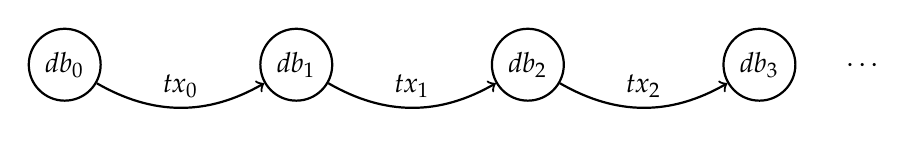
\begin{tikzpicture}[state/.style={circle, draw=black}]
\begin{scope}[thick]
  \node[state]   (db0)                      {$\mathit{db}_0$};
  \node[state]   (db1) [right=2.0cm of db0] {$\mathit{db}_1$};
  \node[state]   (db2) [right=2.0cm of db1] {$\mathit{db}_2$};
  \node[state]   (db3) [right=2.0cm of db2] {$\mathit{db}_3$};
  \node                [right=0.5cm of db3] {$\ldots$};

  \path[->] (db0) edge [bend right] node[above] {$\mathit{tx}_0$} (db1);
  \path[->] (db1) edge [bend right] node[above] {$\mathit{tx}_1$} (db2);
  \path[->] (db2) edge [bend right] node[above] {$\mathit{tx}_2$} (db3);
\end{scope}
\end{tikzpicture}
\begin{align*}
 \mathit{db}_1 & = \mathit{tx}_0(\mathit{db}_0) \\
 \mathit{db}_2 & = \mathit{tx}_1(\mathit{db}_1) \\
 \vdots
\end{align*}
\end{center}
This model serves as an important semantic reference point for the more
complicated models below. we will want to show that some of our more
complicated models are semantically equivalent to this simple one.

If we think of this model in terms of what kind of implementation strategy it
most clearly represents, then it would probably be a simple in-memory design.
That is a design where the whole database is a simple program value that is
transformed with pure functions.

\subsection{Change-based databases}

In this model we want to introduce two concepts
\begin{enumerate}
\item the use of transaction difference functions and applying differences; and
\item identifying the subset of values that each transaction needs.
\end{enumerate}
It is otherwise just a simple sequence of changes. The use of these two concepts
makes this a simple but reasonable model of an on-disk database with in-memory
transaction processing. That is, a database where the data is stored on disk
but all transaction processing is performed on in-memory data structures. Using
a subset of values corresponds to reading the data in from disk, while obtaining
and applying differences corresponds to writing changes back to disk.

Whereas in the previous model we had a series of transaction functions
$\mathit{tx}_0, \mathit{tx}_1, \ldots$, in this model we will have difference
functions
$\delta\mathit{tx}_0, \delta\mathit{tx}_1, \ldots : \mathit{DB} \to \Delta\mathit{DB}$. These are required to be proper difference functions, obeying the property
\begin{equation}
\label{eq:diff-fun}
db \triangleleft \delta\mathit{tx}(\mathit{db}) = \mathit{tx}(\mathit{db})
\end{equation}

For each transaction we will also identify the subset of the database state that
the transaction needs. This will typically take the form of a set of keys
$\mathit{ks} \in \dom{\mathit{DB}}$ (or collection of sets of keys) and
performing a domain restriction $\restrict{\mathit{db}}{\mathit{ks}} \in \mathit{DB}$.
So there will key sets $\mathit{ks}_0, \mathit{ks}_1, \ldots$ corresponding to
the transactions $\delta\mathit{tx}_0, \delta\mathit{tx}_1, \ldots$.
We will require that the transaction really does only make use of the subset
by requiring the property that the transaction function gives the same result
on the subset as the whole state
\begin{equation}
\label{eq:restrict}
  \delta\mathit{tx}_i(\restrict{\mathit{db}}{\mathit{ks}_i}) = \delta\mathit{tx}_i(\mathit{db})
\end{equation}
A lemma that will prove useful later is that domain restriction commutes with
applying changes
\begin{equation}
\label{eq:restriction}
  \restrict{\mathit{db}}{\mathit{ks}} \triangleleft \delta\mathit{db}
=
  \restrict{\left(\mathit{db} \triangleleft \delta\mathit{db}\right)}{\mathit{ks}}
\end{equation}
This lemma either needs to be proved universally or we will need to make it a
required property of the differences.

We can now construct the series of database states
$\mathit{db}_0, \mathit{db}_1, \ldots$
by applying the changes from each transaction to the previous database state.

\begin{center}
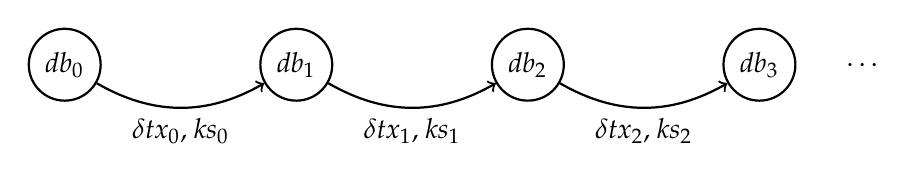
\begin{tikzpicture}[state/.style={circle, draw=black}]
\begin{scope}[thick]
  \node[state]   (db0)                      {$\mathit{db}_0$};
  \node[state]   (db1) [right=2.0cm of db0] {$\mathit{db}_1$};
  \node[state]   (db2) [right=2.0cm of db1] {$\mathit{db}_2$};
  \node[state]   (db3) [right=2.0cm of db2] {$\mathit{db}_3$};
  \node                [right=0.5cm of db3] {$\ldots$};

  \path[->] (db0) edge [bend right] node[below] {$\delta\mathit{tx}_0$, $\mathit{ks}_0$} (db1);
  \path[->] (db1) edge [bend right] node[below] {$\delta\mathit{tx}_1$, $\mathit{ks}_1$} (db2);
  \path[->] (db2) edge [bend right] node[below] {$\delta\mathit{tx}_2$, $\mathit{ks}_2$} (db3);
\end{scope}
\end{tikzpicture}
\begin{align*}
 \mathit{db}_1 & = \mathit{db}_0 \triangleleft \delta\mathit{tx}_0(\restrict{\mathit{db}_0}{\mathit{ks}_0}) \\
 \mathit{db}_2 & = \mathit{db}_1 \triangleleft \delta\mathit{tx}_1(\restrict{\mathit{db}_1}{\mathit{ks}_1}) \\
 \vdots
\end{align*}
\end{center}
It is straightforward to see how this is equivalent to the simple model.
\begin{align*}
       & \mathit{db}_{i+1} = \mathit{db}_i \triangleleft \delta\mathit{tx}_i(\restrict{\mathit{db}_i}{\mathit{ks}_i}) \\
\equiv & \quad \text{\{by the restriction property \cref{eq:restrict} that
                     $\delta\mathit{tx}_i(\restrict{\mathit{db}}{\mathit{ks}_i}) = \delta\mathit{tx}_i(\mathit{db})$\}} \\
       & \mathit{db}_{i+1} = \mathit{db}_i \triangleleft \delta\mathit{tx}_i(\mathit{db}_i) \\
\equiv & \quad \text{\{by the difference function property \cref{eq:diff-fun} that
                     $db \triangleleft \delta\mathit{tx}(\mathit{db}) = \mathit{tx}(\mathit{db})$\}} \\
       & \mathit{db}_{i+1} = \mathit{tx}_i(\mathit{db}_i)
\end{align*}
And hence, just as in the simple model, it is the case that
\begin{align*}
 \mathit{db}_1 & = \mathit{tx}_0(\mathit{db}_0) \\
 \mathit{db}_2 & = \mathit{tx}_1(\mathit{db}_1) \\
 \vdots
\end{align*}


\subsection{Change-based pipelined databases}

Here is where things start to get interesting and tricky. As discussed in
\cref{enabling-pipelining} we wish to pipeline reads from disk to provide the
opportunity to use parallel I/O. Providing this opportunity is not something
that we can hide, and it will have to be explicit in how we manage the logical
state of the database. So the purpose of this model is to provide a reasonable
correspond to an implementation that could use pipelined reads. We will also
want to show that it is nevertheless mathematically equivalent to the simple
model.

The goal with the pipelining of I/O reads is to initiate the I/O operations
early so the results are already available in memory by the time they are
needed later. This allows the I/O to be overlapped with computation, and it
also allows a substantial number of I/O operations to be in progress at once,
which is what provides the opportunity to use parallel I/O.

The difficulty however is that initiating the reads early means that the state
of the database in which we initiated the reads is not necessarily the same
state as the one in which we use the read results to perform a transaction.
In the diagram below we see an example where a read of key set $\mathit{ks}_1$
is performed against database state $\mathit{db}_0$ to give us a read set
$\mathit{rs}_1 = \restrict{\mathit{db}_0}{\mathit{ks}_1}$. The transaction
$\delta\mathit{tx}_1$ using this read set $\mathit{rs}_1$ is being applied
starting from database state $\mathit{db}_1$ which is \emph{not} the same as
the database state $\mathit{db}_0$ the read was performed against. Any updates
applied in $\mathit{db}_1$ that might affect $\mathit{rs}_1$ would be lost and
we would get the wrong result.
\begin{center}
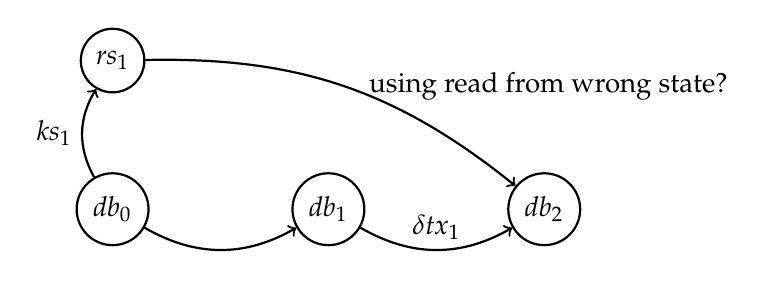
\begin{tikzpicture}[state/.style={circle, draw=black}]
\begin{scope}[thick]
  \node[state]   (db0)                      {$\mathit{db}_0$};
  \node[state]   (db1) [right=1.8cm of db0] {$\mathit{db}_1$};
  \node[state]   (db2) [right=1.8cm of db1] {$\mathit{db}_2$};

  \node[state]   (rs1) [above=1.0cm of db0] {$\mathit{rs}_1$};

  \path[->] (db0) edge [bend left] node[left] {$\mathit{ks}_1$} (rs1);

  \path[->] (rs1) edge [bend left=20] node[right=0.2cm] {using read from wrong state?} (db2);

  \path[->] (db0) edge [bend right] node[above] {} (db1);
  \path[->] (db1) edge [bend right] node[above] {$\delta\mathit{tx}_1$} (db2);
\end{scope}
\end{tikzpicture}
\end{center}
Contrast this with the model in the previous section. That model uses `reads'
from the database (modelled as $\restrict{\mathit{db}_i}{\mathit{ks}_i}$) but
the reads are done from the same database state as the transaction itself.

Apparently with pipelining we no longer have straightforwardly sequential state
updates. Of course pipelining is only acceptable if can find some way to make
it semantically equivalent to the sequential version.

\begin{center}
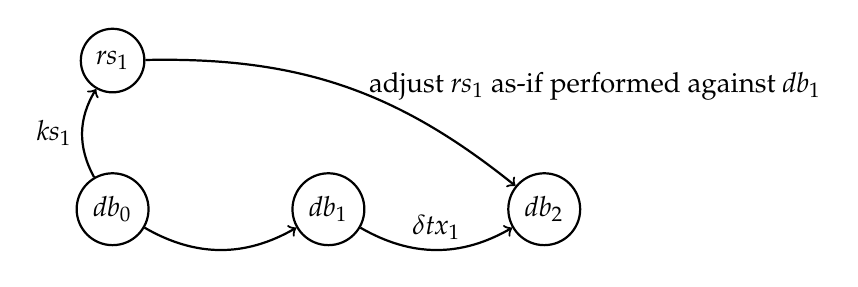
\begin{tikzpicture}[state/.style={circle, draw=black}]
\begin{scope}[thick]
  \node[state]   (db0)                      {$\mathit{db}_0$};
  \node[state]   (db1) [right=1.8cm of db0] {$\mathit{db}_1$};
  \node[state]   (db2) [right=1.8cm of db1] {$\mathit{db}_2$};

  \node[state]   (rs1) [above=1.0cm of db0] {$\mathit{rs}_1$};

  \path[->] (db0) edge [bend left] node[left] {$\mathit{ks}_1$} (rs1);

  \path[->] (rs1) edge [bend left=20] node[right=0.2cm] {adjust $\mathit{rs}_1$ as-if performed against $\mathit{db}_1$} (db2);

  \path[->] (db0) edge [bend right] node[above] {} (db1);
  \path[->] (db1) edge [bend right] node[above] {$\delta\mathit{tx}_1$} (db2);
\end{scope}
\end{tikzpicture}
\end{center}
The trick to restoring equivalence to the sequential version is to adjust the
result of the reads so that it is as if they had been performed against the
right state of the database.

We observed before that the problem was that any updates applied in
$\mathit{db}_1$ that might affect $\mathit{rs}_1$ would be lost. Since we are
working with differences we of course know \emph{exactly} what changes were
applied to $\mathit{db}_1$. We can apply those same changes to the read set
$\mathit{rs}_1$. In the example above those changes are exactly the ones
performed by the previous transaction $\delta\mathit{tx}_0$.

More generally the changes we want to apply are all those that occurred between
the state against which the read was performed and the state in which the
transaction using the read results is to be applied. Thus in our designs we
will have to carefully track and apply the changes from where a read was
initiated to where it is used.

If we can do so successfully however it seems clear that we can obtain a
arbitrary depths of pipelining, at the memory cost of tracking the intervening
changes. In the diagram below we illustrate a series of transactions using
pipelined reads with a fixed depth of one.
\begin{center}
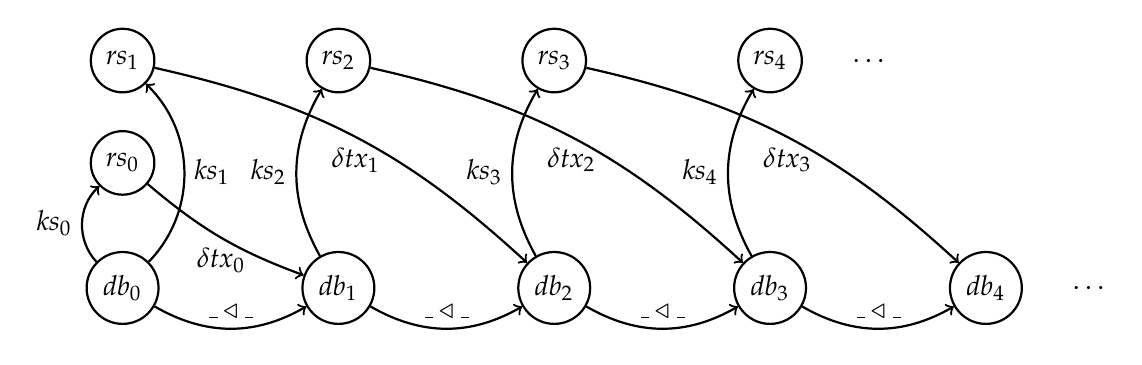
\begin{tikzpicture}[state/.style={circle, draw=black}]
\begin{scope}[thick]
  \node[state]   (db0)                      {$\mathit{db}_0$};
  \node[state]   (db1) [right=1.8cm of db0] {$\mathit{db}_1$};
  \node[state]   (db2) [right=1.8cm of db1] {$\mathit{db}_2$};
  \node[state]   (db3) [right=1.8cm of db2] {$\mathit{db}_3$};
  \node[state]   (db4) [right=1.8cm of db3] {$\mathit{db}_4$};
  \node                [right=0.5cm of db4] {$\ldots$};

  \node[state]   (rs0) [above=0.7cm of db0] {$\mathit{rs}_0$};
  \node[state]   (rs1) [above=2.0cm of db0] {$\mathit{rs}_1$};
  \node[state]   (rs2) [above=2.0cm of db1] {$\mathit{rs}_2$};
  \node[state]   (rs3) [above=2.0cm of db2] {$\mathit{rs}_3$};
  \node[state]   (rs4) [above=2.0cm of db3] {$\mathit{rs}_4$};
  \node                [right=0.5cm of rs4] {$\ldots$};

  \path[->] (db0) edge [bend left=45]  node[left]  {$\mathit{ks}_0$} (rs0);
  \path[->] (db0) edge [bend right=45] node[right] {$\mathit{ks}_1$} (rs1);
  \path[->] (db1) edge [bend left]     node[left]  {$\mathit{ks}_2$} (rs2);
  \path[->] (db2) edge [bend left]     node[left]  {$\mathit{ks}_3$} (rs3);
  \path[->] (db3) edge [bend left]     node[left]  {$\mathit{ks}_4$} (rs4);

  \path[->] (rs0) edge [bend right=10] node[below] {$\delta\mathit{tx}_0$} (db1);
  \path[->] (rs1) edge [bend left=15]  node[below] {$\delta\mathit{tx}_1$} (db2);
  \path[->] (rs2) edge [bend left=15]  node[below] {$\delta\mathit{tx}_2$} (db3);
  \path[->] (rs3) edge [bend left=15]  node[below] {$\delta\mathit{tx}_3$} (db4);

  \path[->] (db0) edge [bend right] node[above] {$\_ \triangleleft \_$} (db1);
  \path[->] (db1) edge [bend right] node[above] {$\_ \triangleleft \_$} (db2);
  \path[->] (db2) edge [bend right] node[above] {$\_ \triangleleft \_$} (db3);
  \path[->] (db3) edge [bend right] node[above] {$\_ \triangleleft \_$} (db4);
\end{scope}
\end{tikzpicture}
\begin{equation*}
\begin{array}{c@{\quad}l@{\quad}l}
    \mathit{db}_1 = \mathit{db}_0 \triangleleft \delta\mathit{db}_0
  & \mathbf{where} \quad \delta\mathit{db}_0 = \delta\mathit{tx}_0(\mathit{rs}_0)
  & \mathbf{and}   \quad \mathit{rs}_0 = \restrict{\mathit{db}_0}{\mathit{ks}_0}
\\
    \mathit{db}_2 = \mathit{db}_1 \triangleleft \delta\mathit{db}_1
  & \mathbf{where} \quad \delta\mathit{db}_1 = \delta\mathit{tx}_1\left(\restrict{(\mathit{rs}_1 \triangleleft \delta\mathit{db}_0)}{\mathit{ks}_1}\right)
  & \mathbf{and}   \quad \mathit{rs}_1 = \restrict{\mathit{db}_0}{\mathit{ks}_1}
\\
    \mathit{db}_3 = \mathit{db}_2 \triangleleft \delta\mathit{db}_2
  & \mathbf{where} \quad \delta\mathit{db}_2 = \delta\mathit{tx}_2\left(\restrict{(\mathit{rs}_2 \triangleleft \delta\mathit{db}_1)}{\mathit{ks}_2}\right)
  & \mathbf{and}   \quad \mathit{rs}_2 = \restrict{\mathit{db}_1}{\mathit{ks}_2}
\\
 \vdots
\end{array}
\end{equation*}
\end{center}
We need to clarify how exactly this is equivalent to the simple sequential
model. We now have a more interesting recurrence relation than in previous
models so we argue by induction. Due to the setup step for the pipelining, we
start from $i=1$ rather than $i=0$.
\begin{align*}
       & \mathit{db}_{i+1} = \mathit{db}_i \triangleleft \delta\mathit{db}_i
         \quad \mathbf{where} \quad \delta\mathit{db}_i = \delta\mathit{tx}_i\left(\restrict{\left(\mathit{rs}_i \triangleleft \delta\mathit{db}_{i-1}\right)}{\mathit{ks}_i}\right)
         \quad \mathbf{and} \quad \mathit{rs}_i = \restrict{\mathit{db}_{i-1}}{\mathit{ks}_i}
      \\
\equiv & \quad \text{\{by substitution of $\mathit{rs}_i$ \}}
      \\
       & \mathit{db}_{i+1} = \mathit{db}_i \triangleleft \delta\mathit{db}_i
         \quad \mathbf{where} \quad \delta\mathit{db}_i = \delta\mathit{tx}_i\left(\restrict{\left(\restrict{\mathit{db}_{i-1}}{\mathit{ks}_i} \triangleleft \delta\mathit{db}_{i-1}\right)}{\mathit{ks}_i}\right)
      \\
\equiv & \quad \text{\{by the domain restriction lemma \cref{eq:restriction}, and idempotency of restriction \}}
      \\
       & \mathit{db}_{i+1} = \mathit{db}_i \triangleleft \delta\mathit{db}_i
         \quad \mathbf{where} \quad \delta\mathit{db}_i = \delta\mathit{tx}_i\left(\restrict{\left(\mathit{db}_{i-1} \triangleleft \delta\mathit{db}_{i-1}\right)}{\mathit{ks}_i}\right)
      \\
\equiv & \quad \text{\{by induction hypothesis $\mathit{db}_i = \mathit{db}_{i-1} \triangleleft \delta\mathit{db}_{i-1}$ \}}
      \\
       & \mathit{db}_{i+1} = \mathit{db}_i \triangleleft \delta\mathit{db}_i
         \quad \mathbf{where} \quad \delta\mathit{db}_i = \delta\mathit{tx}_i\left(\restrict{\mathit{db}_i}{\mathit{ks}_i}\right)
      \\
\equiv & \quad \text{\{by substitution of $\delta\mathit{db}_i$\}}
      \\
       & \mathit{db}_{i+1} = \mathit{db}_i \triangleleft \delta\mathit{tx}_i(\restrict{\mathit{db}_i}{\mathit{ks}_i})
      \\
\equiv & \quad \text{\{by the restriction property \cref{eq:restrict} that
                     $\delta\mathit{tx}_i(\restrict{\mathit{db}}{\mathit{ks}_i}) = \delta\mathit{tx}_i(\mathit{db})$\}}
      \\
       & \mathit{db}_{i+1} = \mathit{db}_i \triangleleft \delta\mathit{tx}_i(\mathit{db}_i)
      \\
\equiv & \quad \text{\{by the difference function property \cref{eq:diff-fun} that
                     $db \triangleleft \delta\mathit{tx}(\mathit{db}) = \mathit{tx}(\mathit{db})$\}}
      \\
       & \mathit{db}_{i+1} = \mathit{tx}_i(\mathit{db}_i)
\end{align*}

\subsection{Hybrid on-disk / in-memory databases}
\label{sec:hybrid-on-disk-in-memory-db}

In this model we go back to a sequential style for simplicity, but we represent
the data as a combination of two parts. One will stand for data on disk and the
other will stand for data in memory. The part on disk will be ordinary database
values $\mathit{db}^{\mathrm{disk}}_i \in \mathit{DB}$, while the part in
memory will be database differences
$\delta\mathit{db}^{\mathrm{mem}}_i \in \Delta\mathit{DB}$. We
define the  overall logical value of the database to be the on-disk part with
the in-memory changes applied on top.
\[
\mathit{db}_i = \mathit{db}^{\mathrm{disk}}_i \triangleleft \delta\mathit{db}^{\mathrm{mem}}_i
\]
\begin{center}
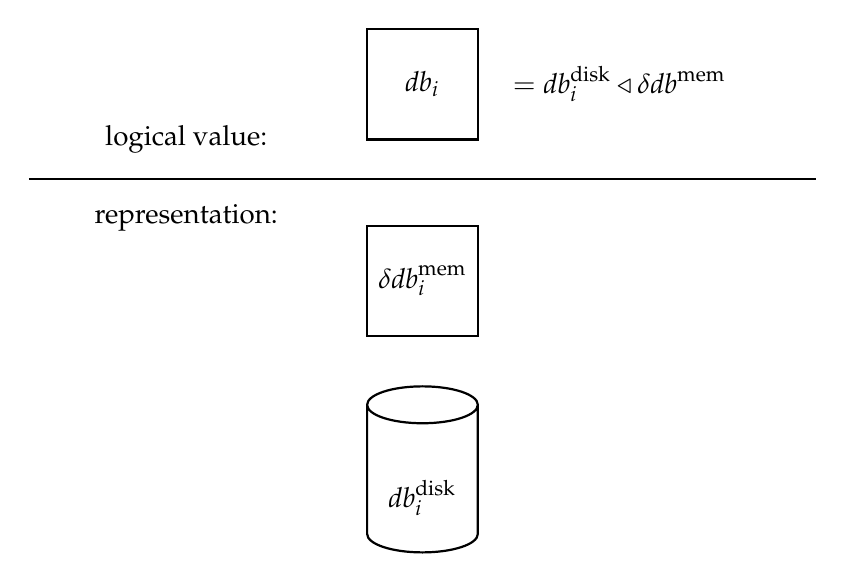
\begin{tikzpicture}[state/.style={circle, draw=black}]
\begin{scope}[thick]

  % disk icon
  \node[cylinder, aspect=2, rotate=90, draw, minimum height=60pt, minimum width=40pt]
        at (0,-25pt) {};
  \draw (0, -30pt) node {$\mathit{db}^{\mathrm{disk}}_i$};

  % in memory
  \draw (-20pt,1) rectangle (20pt,1cm+40pt);
  \draw (0,1cm+20pt) node {$\delta\mathit{db}^{\mathrm{mem}}_i$};

  % dividing line
  \draw (-5,3) -- (5,3);
  \draw (-3,3.5) node {logical value:};
  \draw (-3,2.5) node {representation:};

  % logical value
  \draw (-20pt,3.5cm) rectangle (20pt,3.5cm+40pt);
  \draw (0,3.5cm+20pt) node {$\mathit{db}_i$};
  \draw (2.5,3.5cm+20pt) node {$ = \mathit{db}^{\mathrm{disk}}_i \triangleleft \delta\mathit{db}^{\mathrm{mem}}$};
\end{scope}
\end{tikzpicture}
\end{center}
We now need to see how performing transactions works in this representation. We
will of course use the change-based style of transactions. Given the changes
made by a transaction $\delta\mathit{tx}_i(\restrict{\mathit{db}_i}{\mathit{ks}_i})$
we would normally obtain the new state of the database by applying the changes
to the previous state
\[
\mathit{db}_{i+1} = \mathit{db}_i \triangleleft \delta\mathit{tx}_i(\restrict{\mathit{db}_i}{\mathit{ks}_i})
\]
With the hybrid representation that is
\[
\mathit{db}_{i+1} = \left( \mathit{db}^{\mathrm{disk}}_i \triangleleft \delta\mathit{db}^{\mathrm{mem}}_i \right)
      \triangleleft \delta\mathit{tx}_i(\restrict{\mathit{db}_i}{\mathit{ks}_i})
\]
As we know from \cref{eq:apply-compose}, applying two sets of changes is
equivalent to applying the composition of the changes, and we choose to make
use of this.
\[
\mathit{db}_{i+1} = \mathit{db}^{\mathrm{disk}}_i
      \triangleleft \left( \delta\mathit{db}^{\mathrm{mem}}_i
                  \diamond \delta\mathit{tx}_i(\restrict{\mathit{db}_i}{\mathit{ks}_i})
                    \right)
\]
This now fits the same hybrid representation. We can define the new in-memory
value to be
\[
\delta\mathit{db}^{\mathrm{mem}}_{i+1} = \delta\mathit{db}^{\mathrm{mem}}_i
                  \diamond \delta\mathit{tx}_i(\restrict{\mathit{db}_i}{\mathit{ks}_i})
\]
to get
\[
\mathit{db}_{i+1} = \mathit{db}^{\mathrm{disk}}_i
      \triangleleft \delta\mathit{db}^{\mathrm{mem}}_{i+1}
\]
Or pictorally
\begin{center}
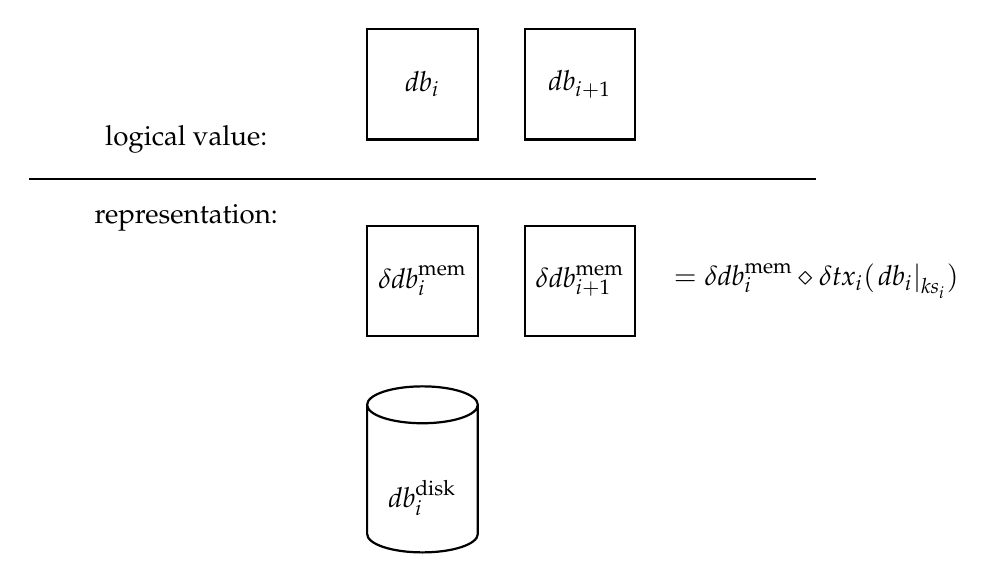
\begin{tikzpicture}[state/.style={circle, draw=black}]
\begin{scope}[thick]

  % disk icon
  \node[cylinder, aspect=2, rotate=90, draw, minimum height=60pt, minimum width=40pt]
        at (0,-25pt) {};
  \draw (0, -30pt) node {$\mathit{db}^{\mathrm{disk}}_i$};

  % in memory
  \draw (-20pt,1) rectangle (20pt,1cm+40pt);
  \draw (0,1cm+20pt) node {$\delta\mathit{db}^{\mathrm{mem}}_i$};

  \draw (2cm-20pt,1) rectangle (2cm+20pt,1cm+40pt);
  \draw (2cm,1cm+20pt) node {$\delta\mathit{db}^{\mathrm{mem}}_{i+1}$};
  \draw (5,1cm+20pt) node {$ = \delta\mathit{db}^{\mathrm{mem}}_i
                  \diamond \delta\mathit{tx}_i(\restrict{\mathit{db}_i}{\mathit{ks}_i})$};

  % dividing line
  \draw (-5,3) -- (5,3);
  \draw (-3,3.5) node {logical value:};
  \draw (-3,2.5) node {representation:};

  % logical value
  \draw (-20pt,3.5cm) rectangle (20pt,3.5cm+40pt);
  \draw (0,3.5cm+20pt) node {$\mathit{db}_i$};
  \draw (2cm-20pt,3.5cm) rectangle (2cm+20pt,3.5cm+40pt);
  \draw (2,3.5cm+20pt) node {$\mathit{db}_{i+1}$};
\end{scope}
\end{tikzpicture}
\end{center}
Notice that we have applied the transaction exclusively to the in-memory part,
without changing the on-disk part. Obviously we cannot do this indefinitely or
the part kept in memory will grow without bound.

In this approach we must changes to disk from time to time flush. Let us see
how that might work. Of course flushing is not supposed to change the logical
value of the database, just to shuffle data from the in-memory part to the
on-disk part. Suppose we start from a state
\[
\mathit{db} = \mathit{db}^{\mathrm{disk}}
      \triangleleft \delta\mathit{db}^{\mathrm{mem}}
\]
We can in principle split the in-memory part into the composition of two sets
of changes.
\[
\delta\mathit{db}^{\mathrm{mem}} = \delta\mathit{db}^{\mathrm{mem}}_a \diamond \delta\mathit{db}^{\mathrm{mem}}_b
\]
The idea is that the first part will be flushed to disk and the second part
will remain in memory. We have a lot of choice here. We can split this in any
way we like. We could choose to flush everything to disk for example, by picking
$\delta\mathit{db}^{\mathrm{mem}}_b = \mathbf{0}$, but we can also choose to
flush just a subset of changes.

Doing the flush is another straightforward application of
\cref{eq:apply-compose}, but in the opposite direction.
\begin{align*}
       & \mathit{db} = \mathit{db}^{\mathrm{disk}}
         \triangleleft \left( \delta\mathit{db}^{\mathrm{mem}}_a \diamond \delta\mathit{db}^{\mathrm{mem}}_b \right)
\\
\equiv & \\
       & \mathit{db} = \left(\mathit{db}^{\mathrm{disk}}
      \triangleleft \delta\mathit{db}^{\mathrm{mem}}_a \right) \triangleleft \delta\mathit{db}^{\mathrm{mem}}_b
\end{align*}
We can interpret the application of changes
$\mathit{db}^{\mathrm{disk}} \triangleleft \delta\mathit{db}^{\mathrm{mem}}_a$
as performing the writes to the on-disk database.
Here is the same in pictorial style:
\begin{center}
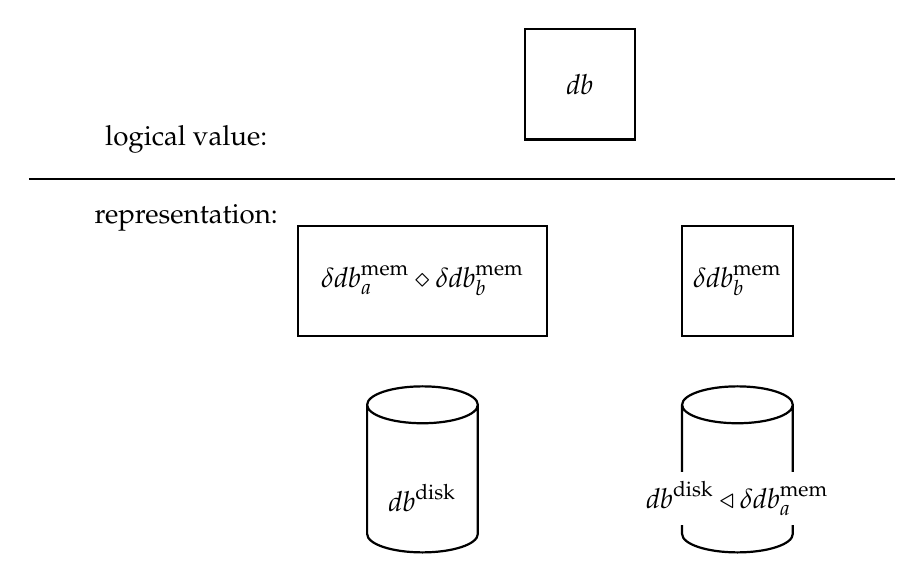
\begin{tikzpicture}[state/.style={circle, draw=black}]
\begin{scope}[thick]

  % disk icon
  \begin{scope}[]
  \node[cylinder, aspect=2, rotate=90, draw, minimum height=60pt, minimum width=40pt]
        at (0,-25pt) {};
  \draw (0, -30pt) node {$\mathit{db}^{\mathrm{disk}}$};
  \end{scope}

  \begin{scope}[xshift=4cm]
  \node[cylinder, aspect=2, rotate=90, draw, minimum height=60pt, minimum width=40pt]
        at (0,-25pt) {};
  \draw (0, -30pt) node[fill=white] {$\mathit{db}^{\mathrm{disk}} \triangleleft \delta\mathit{db}^{\mathrm{mem}}_a$};
  \end{scope}

  % in memory
  \draw (-45pt,1) rectangle (45pt,1cm+40pt);
  \draw (0,1cm+20pt) node {$\delta\mathit{db}^{\mathrm{mem}}_a \diamond \delta\mathit{db}^{\mathrm{mem}}_b$};

  \draw (4cm-20pt,1) rectangle (4cm+20pt,1cm+40pt);
  \draw (4cm,1cm+20pt) node {$\delta\mathit{db}^{\mathrm{mem}}_b$};

  % dividing line
  \draw (-5,3) -- (6,3);
  \draw (-3,3.5) node {logical value:};
  \draw (-3,2.5) node {representation:};

  % logical value
  \draw (2cm-20pt,3.5cm) rectangle (2cm+20pt,3.5cm+40pt);
  \draw (2cm,3.5cm+20pt) node {$\mathit{db}$};
\end{scope}
\end{tikzpicture}
\end{center}

\subsection{Multiple logical database states}

In the models so far, while we have of course defined many logical values of
a database, we have implicitly assumed that these are the evolving states of
a single database over time. We now wish to model a situation in which we want
to maintain and have efficient access to many logical values of a database at
once.

This corresponds roughly to the situation we have in the consensus design where
it is necessary to have efficient access to ledger states corresponding to the
last K blocks\footnote{On the Cardano mainnet K is 2160, so quite a few}. We
need these ledger states to be able to evaluate the validity of candidate
chains that intersect with our own at any point within the last K blocks. In
the current wholly in-memory consensus design we can maintain K ledger states
at very little additional memory cost compared to a single ledger state. This
takes advantage of persistent data structures. This works because the K ledger
states are very closely related: being the ledger states obtained from applying
a series of blocks.

The idea we want to model here is having a single on-disk state at once, but
a whole series of in-memory differences, giving us a series of logical database
values.

\begin{center}
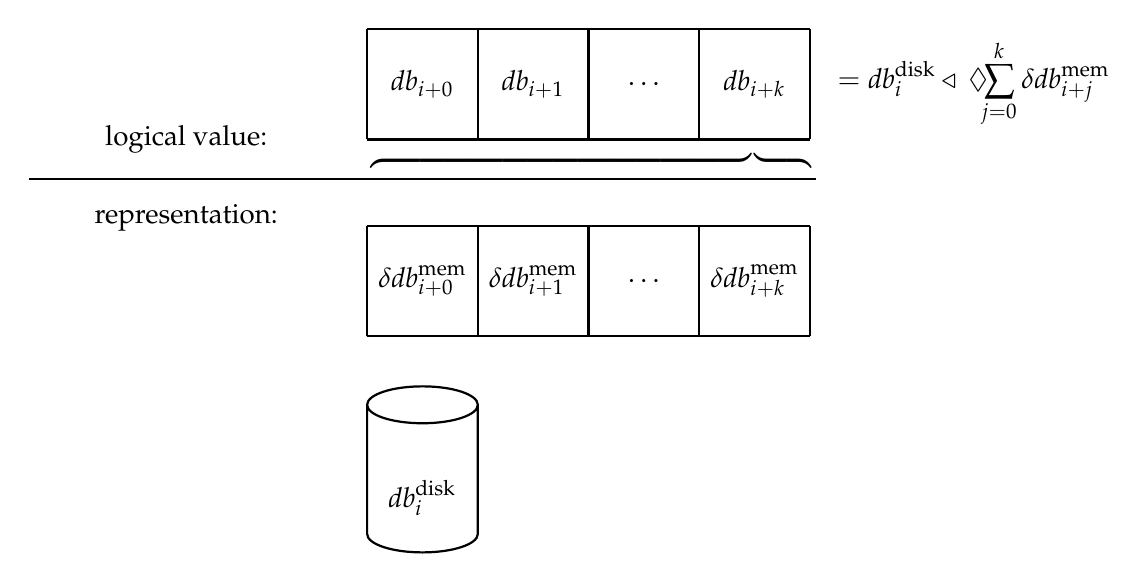
\begin{tikzpicture}[state/.style={circle, draw=black}]
\begin{scope}[thick]

  % disk icon
  \node[cylinder, aspect=2, rotate=90, draw, minimum height=60pt, minimum width=40pt]
        at (0,-25pt) {};
  \draw (0, -30pt) node {$\mathit{db}^{\mathrm{disk}}_i$};

  % in memory
  \draw[step=40pt,xshift=-20pt,yshift=1cm] (0,0) grid (160pt,40pt);
  \draw (0,1cm+20pt) node {$\delta\mathit{db}^{\mathrm{mem}}_{i+0}$};
  \draw (40pt,1cm+20pt)  node {$\delta\mathit{db}^{\mathrm{mem}}_{i+1}$};
  \draw (80pt,1cm+20pt)  node {$\ldots$};
  \draw (120pt,1cm+20pt) node {$\delta\mathit{db}^{\mathrm{mem}}_{i+k}$};

  % dividing line
  \draw (-5,3) -- (5,3);
  \draw (-3,3.5) node {logical value:};
  \draw (-3,2.5) node {representation:};

  % logical value
  \draw[step=40pt,xshift=-20pt,yshift=3.5cm] (0,0) grid (160pt,40pt);
  \draw (0,3.5cm+20pt) node {$\mathit{db}_{i+0}$};
  \draw (40pt,3.5cm+20pt) node {$\mathit{db}_{i+1}$};
  \draw (80pt,3.5cm+20pt) node {$\ldots$};
  \draw (120pt,3.5cm+20pt) node {$\mathit{db}_{i+k}$};

  \node [above delimiter=\rmoustache,
         xshift=50pt,yshift=2.9cm, minimum width=140pt] {};
  \node [above delimiter=\lmoustache,
         xshift=130pt,yshift=2.9cm, minimum width=20pt] {};

  \draw (7,3.5cm+20pt) node
        {$= \mathit{db}^{\mathrm{disk}}_i \triangleleft ~
            \displaystyle\Diamond\hspace{-4pt}\sum_{j=0}^k{\delta\mathit{db}^{\mathrm{mem}}_{i+j}}$};

\end{scope}
\end{tikzpicture}
\end{center}
As depicted in the diagram above, the representation consists of a single disk
state and a series of in-memory differences. Each difference is the individual
difference from performing a transaction. That is, we keep each difference and
do not compose them together prematurely. Then each logical database value is
the value of the on-disk state with the monoidial composition of the appropriate
changes applied on top. That is, for the k\textsuperscript{th} database value
beyond the on disk state we have
\[
\mathit{db}_{i+k}
= \mathit{db}^{\mathrm{disk}}_i \triangleleft ~
            \displaystyle\Diamond\hspace{-4pt}\sum_{j=0}^k{\delta\mathit{db}^{\mathrm{mem}}_{i+j}}
\]
Although we are interested in the compositions of differences we must keep the
individual differences. The reason is that when we do flush changes to disk we
need to discard the oldest in-memory differences which entails computing new
monoidial compositions of the remaining differences.

One interesting implementation idea to manage both a sequence of K differences
and also the efficient monoidial composition of them is to use a \emph{finger
tree} data structure \citep{fingertree}. A finger tree is parametrised over a
monoidal measure. The choice in this case would be both the length and the
differences. The length is the usual measure to support splitting at indexes.
We would rely on splitting to obtain the sub-sequence of differences for
evaluating a chain fork that starts from a recent point on the chain. The other
part of the measure -- the differences -- would mean that the measure of any
sequence or sub-sequence would be the overall monoidal composition of all the
differences in that (sub-)sequence. The finger tree data structure takes care
of efficiently caching the intermediate monoid measure values. Finger trees are
already used extensively within the consensus implementation -- including with
measures other than simply length.

There's a few operations we need to be able to perform in this setting
\begin{enumerate}
\item Perform a transaction. We need to be able to append to the end of the
      sequence of logical database values. This corresponds to adding a block
      to the end of the chain, or adding more transactions to a mempool.
\item Replace any suffix of the sequence of logical database values. This is
      actually a strict generalisation of 1. above. This corresponds to
      switching to a fork, which is a generalisation of appending a single
      block. The replacement sub-sequence can start anywhere in the sequence and
      the replacement can have any length sequence of differences arising from
      blocks.
\item Flush changes to disk. We need to be able to take some of the oldest
      changes and apply them to the disk store.
\end{enumerate}
These operations are straightforward generalisations of the operations we have
already seen in \cref{sec:hybrid-on-disk-in-memory-db}. The first two are about
constructing new logical database values by making new in-memory differences.
In this representation it is simply appending or replacing a suffix of a
sequence of changes. The flushing to disk is a straightforward instance of the
flush operation from \cref{sec:hybrid-on-disk-in-memory-db} where we choose the
a point in the sequence that splits the differences we wish to flush from the
remaining sequence of differences. The value that we apply to the on-disk state
is the monoidal composition of the sequence of differences we wish to flush.

In section ?? we will look at a design for the consensus ledger state
management and chain selection based on the abstract model here, relying only
on the operations we have identified here.

\section{Partial tracking mapping}

In the previous section we assumed that we could find difference functions
$\delta\mathit{tx}$ corresponding to the ordinary transaction functions
$\mathit{tx}$. The correspondence we required was given in \cref{eq:diff-fun},
reproduced here as an aide-m\'emoire:
\begin{equation*}
db \triangleleft \delta\mathit{tx}(\mathit{db}) = \mathit{tx}(\mathit{db})
\end{equation*}


\addcontentsline{toc}{section}{References}
\bibliographystyle{plainnat}
\bibliography{utxo-db}

\end{document}
